\documentclass{scrartcl}
\usepackage{amsmath}
\usepackage{graphicx}
\usepackage{url}
\usepackage{listings}
\renewcommand{\lstlistingname}{Listing}
\title{Polynomial Fitting}
\subtitle{Version 1.0}
\author{R. Steven Turley}
\date{September 1, 2018}
\begin{document}
\maketitle
\tableofcontents

\section{Introduction}
Fitting a polynomial to data is a special case of linear least
squares. Since I discussed that in detail in my Linear Least
Squares article\cite{linLS}, so I won't repeat that information
or those references here except to establish notation. Our goal
is to find the coefficients $b_i$ in the function
\begin{equation}
f(x;\vec{b}) = sum_{k=1}^p b_k x^{k-1}
\end{equation}
that minimize the sum of the squares of the differences between
the function $f$ and the measured data.

\section{Special Polynomial Formulas}
In this section I will specialize the formulas derived in
the Linear Least Squares article\cite{linLS} for polynomials.

\subsection{Finding Fit Parameters}
In order to determine the fit parameters, we need to fill the
matrix $A$ and vector $\vec{v}$ and then solve the matrix equation
\begin{equation}
A\vec{b}=\vec{y}
\end{equation}
for the unknown vector $\vec{b}$ with the fit coefficients.  Since 
the basis functions
\begin{equation}
g_k(x) = x^{k-1}
\end{equation}
the matrix $A$ is
\begin{align}
A &= \left(\begin{array}{ccccc}
n&\sum x_i&\cdots&\sum x_i^{p-2}& \sum x_i^{p-1}\\
\sum x_i& \sum x_i^2 & \cdots &\sum x_i^{p-1} & \sum x_i^p\\
\vdots&\vdots&\vdots\\
\sum x_i^{n-2}&\sum x_i^{n-1}&\cdots&\sum x_i^{n+p-4}& \sum x_i^{n+p-3}\\
\sum x_i^{n-1}&\sum x_i^n&\cdots&\sum x^{n+p-3}&\sum x^{n+p-2}
\end{array}\right)\\
\vec{y} &= \left(\begin{array}{c}
\sum y_i\\
\sum x_i y_i\\
\vdots\\
\sum x_i^{p-2}y_i\\
\sum x_i^{p-1}y_i
\end{array}\right)
\end{align}
The Jacobian needed to find the covariance matrix is
\begin{align}
J_{i,j} &= x_i^{j-1}\\
J &= \left(\begin{array}{ccccc}
1 & x_1 & \cdots & x_1^{p-2} & x_1^{p-1} \\
1 & x_2 & \cdots & x_2^{p-2} & x_2^{p-1} \\
\vdots & \vdots & \vdots & \vdots & \vdots \\
1 & x_{n-1} & \cdots & x_{n-1}^{p-2} & x_{n-1}^{p-1}\\
1 & x_n & \cdots & x_n^{p-2} & x_n^{p-1}
\end{array}\right)\\
J^{T}J &= \left(\begin{array}{ccccc}
\sum x_i^{p-1} & \sum x_i^p & \cdots & \sum x_i^{2p-3} & \sum x_i^{2p-2}\\
\sum x_i^{p-2} & \sum x_i^{p-1} & \cdots & \sum x_i^{2p-4} & \sum x_i^{2p-3}\\
\vdots & \vdots & \vdots & \vdots & \vdots \\
\sum x_i & \sum x_i^2 & \cdots & \sum x_i^{p-1} & \sum x_i^p \\
n & \sum x_i & \cdots & \sum x_i^{p-2} & \sum x_i^{p-1}
\end{array}\right)
\end{align}
As usual, the uncertainties in the fit parameters will be found by
\begin{align}
C &= (J^TJ)^{-21}\\
\sigma_i &= \sigma_y C_{ii}
\end{align}
\section{Using Orthogonal Polynomials}
Polynomials as a sum of monomials are not always be best way to
fit data. The problem is that the quadratic and linear terms can
be highly correlated. Consider fitting the quadratic function
\begin{equation}
y=b_0 + b_1 x + b_2 x^2
\end{equation}
for $b_0 = 2.3$, $b_1 = 1.7$ and $b_2=1.4$ for $0\leq x\leq 1$ with
random noise having an uncertainty of $sigma_y = 0.2$. I used 1,000
data points.

Fig.~\ref{fig:polyfit} is a plot of the data and fit for the polynomial
case.
\begin{figure}
\begin{center}
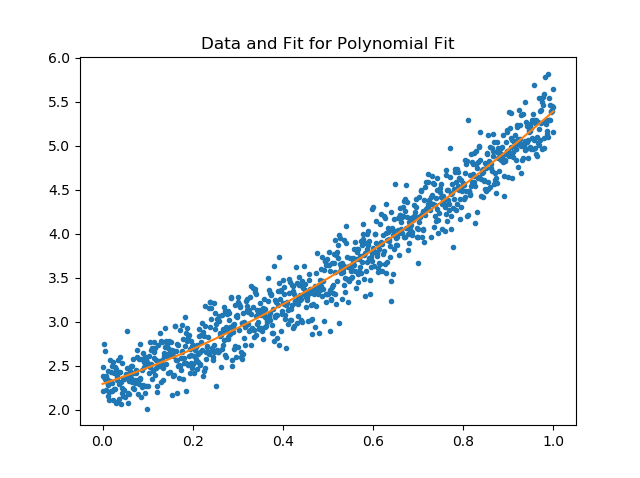
\includegraphics[width=12cm]{polyfit}
\end{center}
\caption{\label{fig:polyfit}Data (blue dots) and the
quadratic polynomial fit to the data (orange line).}
\end{figure}
The fit does a good job following the data and the fit parameters
are good: $b_1=2.29$, $b_2=1.70$, and $b_3=1.40$. However, the
covariance matrix presents problems.
\begin{equation}
C=\left(\begin{array}{ccc}
3.69e-4 & -1.47e-3 & 1.23e-3\\
-1.47e-3 & 7.87 e-3 & -7.38e-3\\
1.23e-3 & -7.38e-3 & 7.38e-3\end{array}\right)
\end{equation}
The off diagonal elements are about the same size as the diagonal
elements. This means the fit parameters are highly correlated with
each other. This can be illustrated further by finding the eigenvectors
of this matrix. Those tell us what linear combinations of monomials
are statistically independent. The eigenvectors are the columns
of the matrix
\begin{equation}
C' = \left(\begin{array}{ccc}
-0.128 & 0.827 & -0.548 \\
0.714 & 0.460 & 0.528 \\
-0.689 & 0.324 & 0.649\end{array}\right)
\end{equation}
Notice that the eigenvectors strongly mix each of the monomial
components.

An alternative is to fit the curve to an expansion in terms
of the ``shifted'' Legendre polynomials which are orthogonal on
the interval $[0,1]$.
\begin{align}
\bar{P}_0(x) &= 1\\
\bar{P}_1(x) &= 2x-1\\
\bar{P}_2(x) &= 6x^2-6x+1
\end{align}
Fitting these values to the data produces a much nicer covariance
matrix.
\begin{equation}
C = \left(\begin{array}{ccc}
4.12e-5 & 3.50e-21 & -2.05e-7\\
3.5e-21 & 1.23e-4 & -1.75e-23\\
-2.05e-7 & -1.75e-23& 2.05e-4\end{array}\right)
\end{equation}
The off-diagonal elements are now much smaller than the diagonal
ones. As one would expect in this case, the eigenvectors
\begin{equation}
C' = \left(\begin{array}{ccc}
-1.000 & -0.000 & -0.001 \\
0.000 & -1.000 & -0.000 \\
-0.001 & 0.000 & 1.000\end{array}\right)
\end{equation}
also show that these coefficients of these polynomials are
statistically independent.
\section{Scaling the Data}
Whether or not you are using orthogonal polynomials, it is a good
idea to express the polynomials in terms of a quantity
$0\leq t\leq 1$. If $x_i\leq x\leq x_f$,
\begin{equation}
t = \frac{x-x_i}{x_f-x_i}
\end{equation}
The coefficients of polynomials in $t$ will be more stable
numerically than polynomials in $x$ if $|x|\gg 1$.

\section{Regression}
A question which arises in polynomial fitting is which terms
make sense to keep statistically. A good way to decide is based
on the Student t distribution. This gives the probability density
that a fit parameter with mean $\mu$ and standard error $\sigma$ will
be $t$ standard deviations away from the origin. Let
$T(t,\nu)$ be the Student t distribution. Then
\begin{equation}
p = 2*\left(1-\int_0^\mu/\sigma T(\tau,\nu)\,d\tau\right)
\end{equation}
which is called the p value is the probability that a fit
parameter value of $\mu$ or greater
could have happened by chance. The parameter $\nu$ is the
number of degrees of freedom in the fit. If $n$ is the number
of data points and $f$ is the number of fit parameters,
\begin{equation}
\nu = n-f
\end{equation}
A good standard for a fit parameter to be statistically significant
is to have $p<0.05$.

\begin{thebibliography}{9}

\bibitem{linLS}
R.~Steven Turley, "Linear Least Squares," BYU, 2018.

\end{thebibliography}

\end{document}
